\documentclass[../../main.tex]{subfiles}
\begin{document}

\begin{flushright}
  \footnotesize\textit{【自動文字起こし・要確認】}
\end{flushright}

{\bf [解答]} (1) $a_n^2 = A_n$ などと表す．与式の分母を払って $(A_0, A_1, B_0, B_1 > 0)$
$$ B_1 (B_0 + 1) + A_1 (A_0 + 1) > A_1 (B_0 + 1) + B_1 (A_0 + 1) $$
を示せば良い．
\begin{align}
  (\text{左辺}) - (\text{右辺}) &= B_1 (B_0 - A_0) + A_1 (A_0 - B_0) \\
  &= (B_1 - A_1) (B_0 - A_0) > 0 \quad (\because A_0 < B_0, A_1 < B_1)
\end{align}
よって示された．

\paragraph{(2)}

$\{x_k\}$ は自然数列 $\{k\}$ の並びかえである．(1) から，$\dfrac{x_i^2}{i^2+1} + \dfrac{x_j^2}{j^2+1} > \dfrac{x_j^2}{i^2+1} + \dfrac{x_i^2}{j^2+1} \; (i < j \in \mathbb{N})$ に対し $x_i < x_j$ なら
だから，$T(n) = \sum_{k=1}^n \dfrac{x_k^2}{k^2+1}$ の値は，$x_i$ と $x_j$ を入れかえた方が小さくなる．したがって，
$k = 1, 2, \cdots$ の順に $x_k$ と $x_m$ $(m = k+1, \cdots, n)$ の大きさを比べ，$x_k < x_m$ ならそのまま，$x_k > x_m$ なる $m$ があるならそのうち $x_m$ が最小のものと $x_k$ を入れかえる作業をすることで，「$x_k = k$」の時，$T(n)$ が $\min$ であることがわかる．
$$ T(n) \ge \sum_{k=1}^n \dfrac{k^2}{k^2+1} = \sum_{k=1}^n \left( 1 - \dfrac{1}{k^2+1} \right) = n - \sum_{k=1}^n \dfrac{1}{k^2+1} \cdots \text{①} $$

ここで，$y = \dfrac{1}{x^2+1}$ のグラフから，面積比較して，
$$ \sum_{k=1}^n \dfrac{1}{k^2+1} \le \dfrac{1}{2} + \int_1^n \dfrac{1}{x^2+1} dx $$

\begin{figure}[htb]
  \centering
  % n=5 の場合．各長方形は右端 x=k における関数値を高さに持つ．
  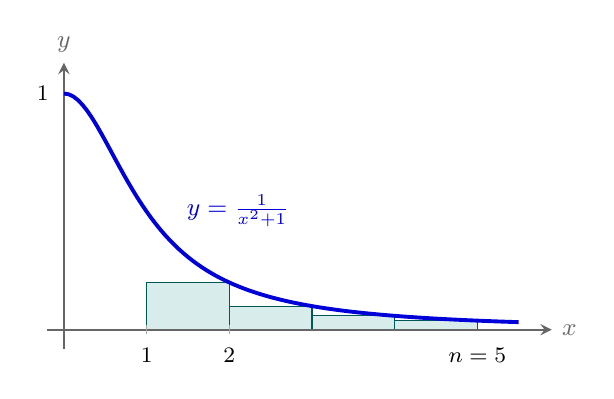
\begin{tikzpicture}[x=1.05cm, y=3cm, >=stealth, every node/.style={font=\small}]
    \foreach \k in {2,...,5} {
      \pgfmathsetmacro{\h}{1/(\k*\k+1)}
      \fill[teal!15] (\k-1,0) rectangle (\k,\h);
      \draw[teal!70!black, thin] (\k-1,0) rectangle (\k,\h);
    }
    \draw[->, thick, gray!80!black] (-0.2,0) -- (5.9,0) node[right] {$x$};
    \draw[->, thick, gray!80!black] (0,-0.08) -- (0,1.13) node[above] {$y$};
    \draw[line width=1.4pt, blue!85!black, domain=0:5.5, samples=100] plot (\x,{1/(\x*\x+1)});
    \foreach \k in {1,2} {
      \draw[gray!70] (\k,0.02) -- (\k,-0.02);
      \node[below=3pt, font=\footnotesize] at (\k,0) {$\k$};
    }
    \node[left=2pt, font=\footnotesize] at (0,1) {$1$};
    \node[above right=2pt, blue!85!black] at (1.3,0.37) {$y=\frac{1}{x^2+1}$};
    \node[below=3pt, font=\footnotesize] at (5,0) {$n=5$};
  \end{tikzpicture}
  \caption{減少する関数と右端を高さにとった長方形の面積比較（図は$n=5$）}
\end{figure}

$\tan \alpha_n = n$ なる $\alpha_n$ を定めると $(0 \le \alpha_n < \pi/2)$
$$ \sum_{k=1}^n \dfrac{1}{k^2+1} \le \dfrac{1}{2} + \alpha_n - \pi/4 $$
①から
$$ T(n) \ge n - \dfrac{1}{2} - \alpha_n + \pi/4 > n - \dfrac{1}{2} - \pi/4 \quad (\because \alpha_n < \pi/2) $$
ここで，$\pi < 3.15 \cdots$ だから，
$$ T(n) > n - \dfrac{1}{2} - \dfrac{3.15}{4} > n - \dfrac{5}{4} $$
$\left( 32 > 25.75 \text{ から } \dfrac{5.15}{4} < \dfrac{5}{4} \right)$

(別解: $\sum \dfrac{1}{k^2+1}$ の評価)
\begin{align}
  \sum_{k=1}^n \dfrac{1}{k^2+1} &< \sum_{k=2}^n \dfrac{1}{k^2-1} + \dfrac{1}{2} = \sum_{k=2}^n \dfrac{1}{2} \left( \dfrac{1}{k-1} - \dfrac{1}{k+1} \right) + \dfrac{1}{2} \\
  &= \dfrac{1}{2} + \dfrac{1}{2} \left( 1 + \dfrac{1}{2} - \dfrac{1}{n} - \dfrac{1}{n+1} \right) \\
  &= \dfrac{5}{4} - \dfrac{1}{2} \left( \dfrac{1}{n} + \dfrac{1}{n+1} \right) < \dfrac{5}{4}
\end{align}

\end{document}
